\documentclass[usenames,dvipsnames, 18pt, compress, aspectratio=169]{beamer}

% can be compiled by xelatex -shell-escape presentation.tex
% lualatex -shell-escape presentation.tex

\usetheme[]{metropolis}

\usepackage[utf8]{inputenc}
\usepackage[russian, english]{babel}
\usepackage{booktabs}
\usepackage[scale=2]{ccicons}
\usepackage{listings}
\usepackage{marvosym}
\usepackage{color}
\usepackage{xcolor}
\usepackage[document]{ragged2e}
\usepackage[export]{adjustbox}
\usepackage{fontawesome}
\usepackage{enumitem}
\usepackage{minted}
\usemintedstyle{tango}
\usepackage[normalem]{ulem}
\usepackage{tikz}
\usetikzlibrary{patterns}
\usetikzlibrary{mindmap}
\usepackage{graphicx}
\usepackage{eso-pic}
\usepackage{verbatim}
\usepackage{smartdiagram}
\usesmartdiagramlibrary{additions}
\usetikzlibrary{trees}
\usepackage{datetime}

\usepackage{tcolorbox}
\usepackage{tabularx}
\usepackage{array}
\usepackage{colortbl}
\tcbuselibrary{skins}

\usetikzlibrary{shapes,arrows,positioning}
\graphicspath{{images/}}
\newfontfamily{\FA}{FontAwesome}

\definecolor{check}{rgb}{0.1,2,0.3}
\definecolor{fail}{rgb}{2,0.1,0.1}
\definecolor{question}{rgb}{0.9,0.9,0.0}

\def\twitter{{\FA \faTwitter}}
\def\github{{\FA \faGithub}}
\def\email{{\FA \faEnvelope}}
\def\check{\textcolor{check}{\FA \faCheck}}
\def\fail{\textcolor{fail}{\FA \faRemove}}
\def\question{\textcolor{question}{\FA \faSearch}}

\renewcommand{\ttdefault}{pcr}
\newfontfamily{\ttfamily}{Fira Code}

\usefonttheme{professionalfonts} % using non standard fonts for beamer
\usefonttheme{serif} % default family is serif
\usepackage{fontspec}
\setmainfont{Liberation Sans}
\newfontfamily\ExtraLight{Liberation Sans}
\newfontfamily\Light{Liberation Sans}
\newfontfamily\Book{Liberation Sans}
\newfontfamily\Medium{Liberation Sans}

\makeatletter
\newcommand\HUGE{\@setfontsize\Huge{32}{41}}
\makeatother

\newcommand\AtPagemyUpperLeft[1]{\AtPageLowerLeft{%
\put(\LenToUnit{0.85\paperwidth},\LenToUnit{0.05\paperheight}){#1}}}

\newcommand\AtPagemyUpperTop[1]{\AtPageLowerLeft{%
\put(\LenToUnit{0.42\paperwidth},\LenToUnit{0.90\paperheight}){#1}}}

\renewcommand{\ULthickness}{2.0pt}

\definecolor{links}{HTML}{0099FF}
\hypersetup{colorlinks, linkcolor=, urlcolor=links}

\setbeamerfont{section title}{family=\Book, size=\Huge, shape=\normalfont}
\setbeamerfont{frametitle}{family=\Book, size=\large, shape=\normalfont}
\setbeamerfont{title}{family=\Book, size=\Large, shape=\normalfont}
\setbeamerfont{subtitle}{size=\small}
\setbeamerfont{author}{family=\ExtraLight, size=\footnotesize}

\newdateformat{specialdate}{\twodigit{\THEDAY}-\twodigit{\THEMONTH}-\THEYEAR}

\newcommand\tikzmark[1]{%
  \tikz[overlay,remember picture] \coordinate (#1);}

\setbeamertemplate{title page}
{

  \vspace*{2.1cm}
  \begin{minipage}[b][\paperheight]{\textwidth}
  \begin{center}

    \ifx\inserttitle\@empty\else
    {{% \inserttitle is nonempty
      \raggedright%
      %\linespread{1.0}%
      \usebeamerfont{title}%
      \usebeamercolor[fg]{title}%
      %\vspace*{1.3em}
      \if@noSmallCapitals%
        \inserttitle%
      \else%
        \scshape{\color{black} \textbf{\begin{center}\inserttitle\end{center}}}%
      \fi%
      \vspace*{0.3em}
    }}
    \fi

    \vspace*{0.5em}%

    \ifx\insertsubtitle\@empty\else
    {{% \insertsubtitle is nonempty
      \usebeamerfont{subtitle}%
      \usebeamercolor[fg]{subtitle}%
      {\color{black} \insertsubtitle}%
      \vspace*{3.0em}%
    }}
    \fi

    \vspace*{1.0em}%

    \usebeamerfont{author}%
    \usebeamercolor[fg]{author}%
    {\color{black} \insertauthor}%

    \vspace*{1.5em}
    \fontsize{8pt}{10}\selectfont
    {\color{black} 20-04-2018}%

    \vfill
    \vspace*{2em}
  \end{center}
  \end{minipage}
}

\setbeamertemplate{section page}
{
  \vspace{2em}
  \centering
  \begin{minipage}{22em}
    \usebeamercolor[fg]{section title}
    \usebeamerfont{section title}
    {\color{black} \insertsectionhead\\[-1ex]}
  \end{minipage}
  \par
}

\setbeamertemplate{footline}
{
\begin{beamercolorbox}[wd=\textwidth,ht=3ex,dp=3ex,leftskip=0.3cm,rightskip=0.3cm]{structure}
  \usebeamerfont{page number in head/foot}
  \insertframenumber
\end{beamercolorbox}
}

\title{POSTGRESQL\\ LINUX KERNEL}
\subtitle{FRIENDSHIP}
\date{\today}
\author{DMITRY DOLGOV}
\institute{}

\begin{document}
{
  \usebackgroundtemplate{
\includegraphics[width=\paperwidth]{template.png}}%
  \fontsize{17pt}{18}\selectfont
  \maketitle
}

\AddToShipoutPictureBG{
  \AtPagemyUpperLeft{{
\includegraphics[width=2.0cm,keepaspectratio]{logo.png}}}
}%

\setbeamertemplate{background canvas}{
\begin{tikzpicture}
    \clip (0,0) rectangle (\paperwidth,\paperheight);
    \fill[color=orange] (4cm, \paperheight-6pt) rectangle (\paperwidth-4cm,\paperheight);
\end{tikzpicture}
}

\fontsize{17pt}{18}\selectfont

\begin{frame}
    \frametitle{}
    \begin{center}

        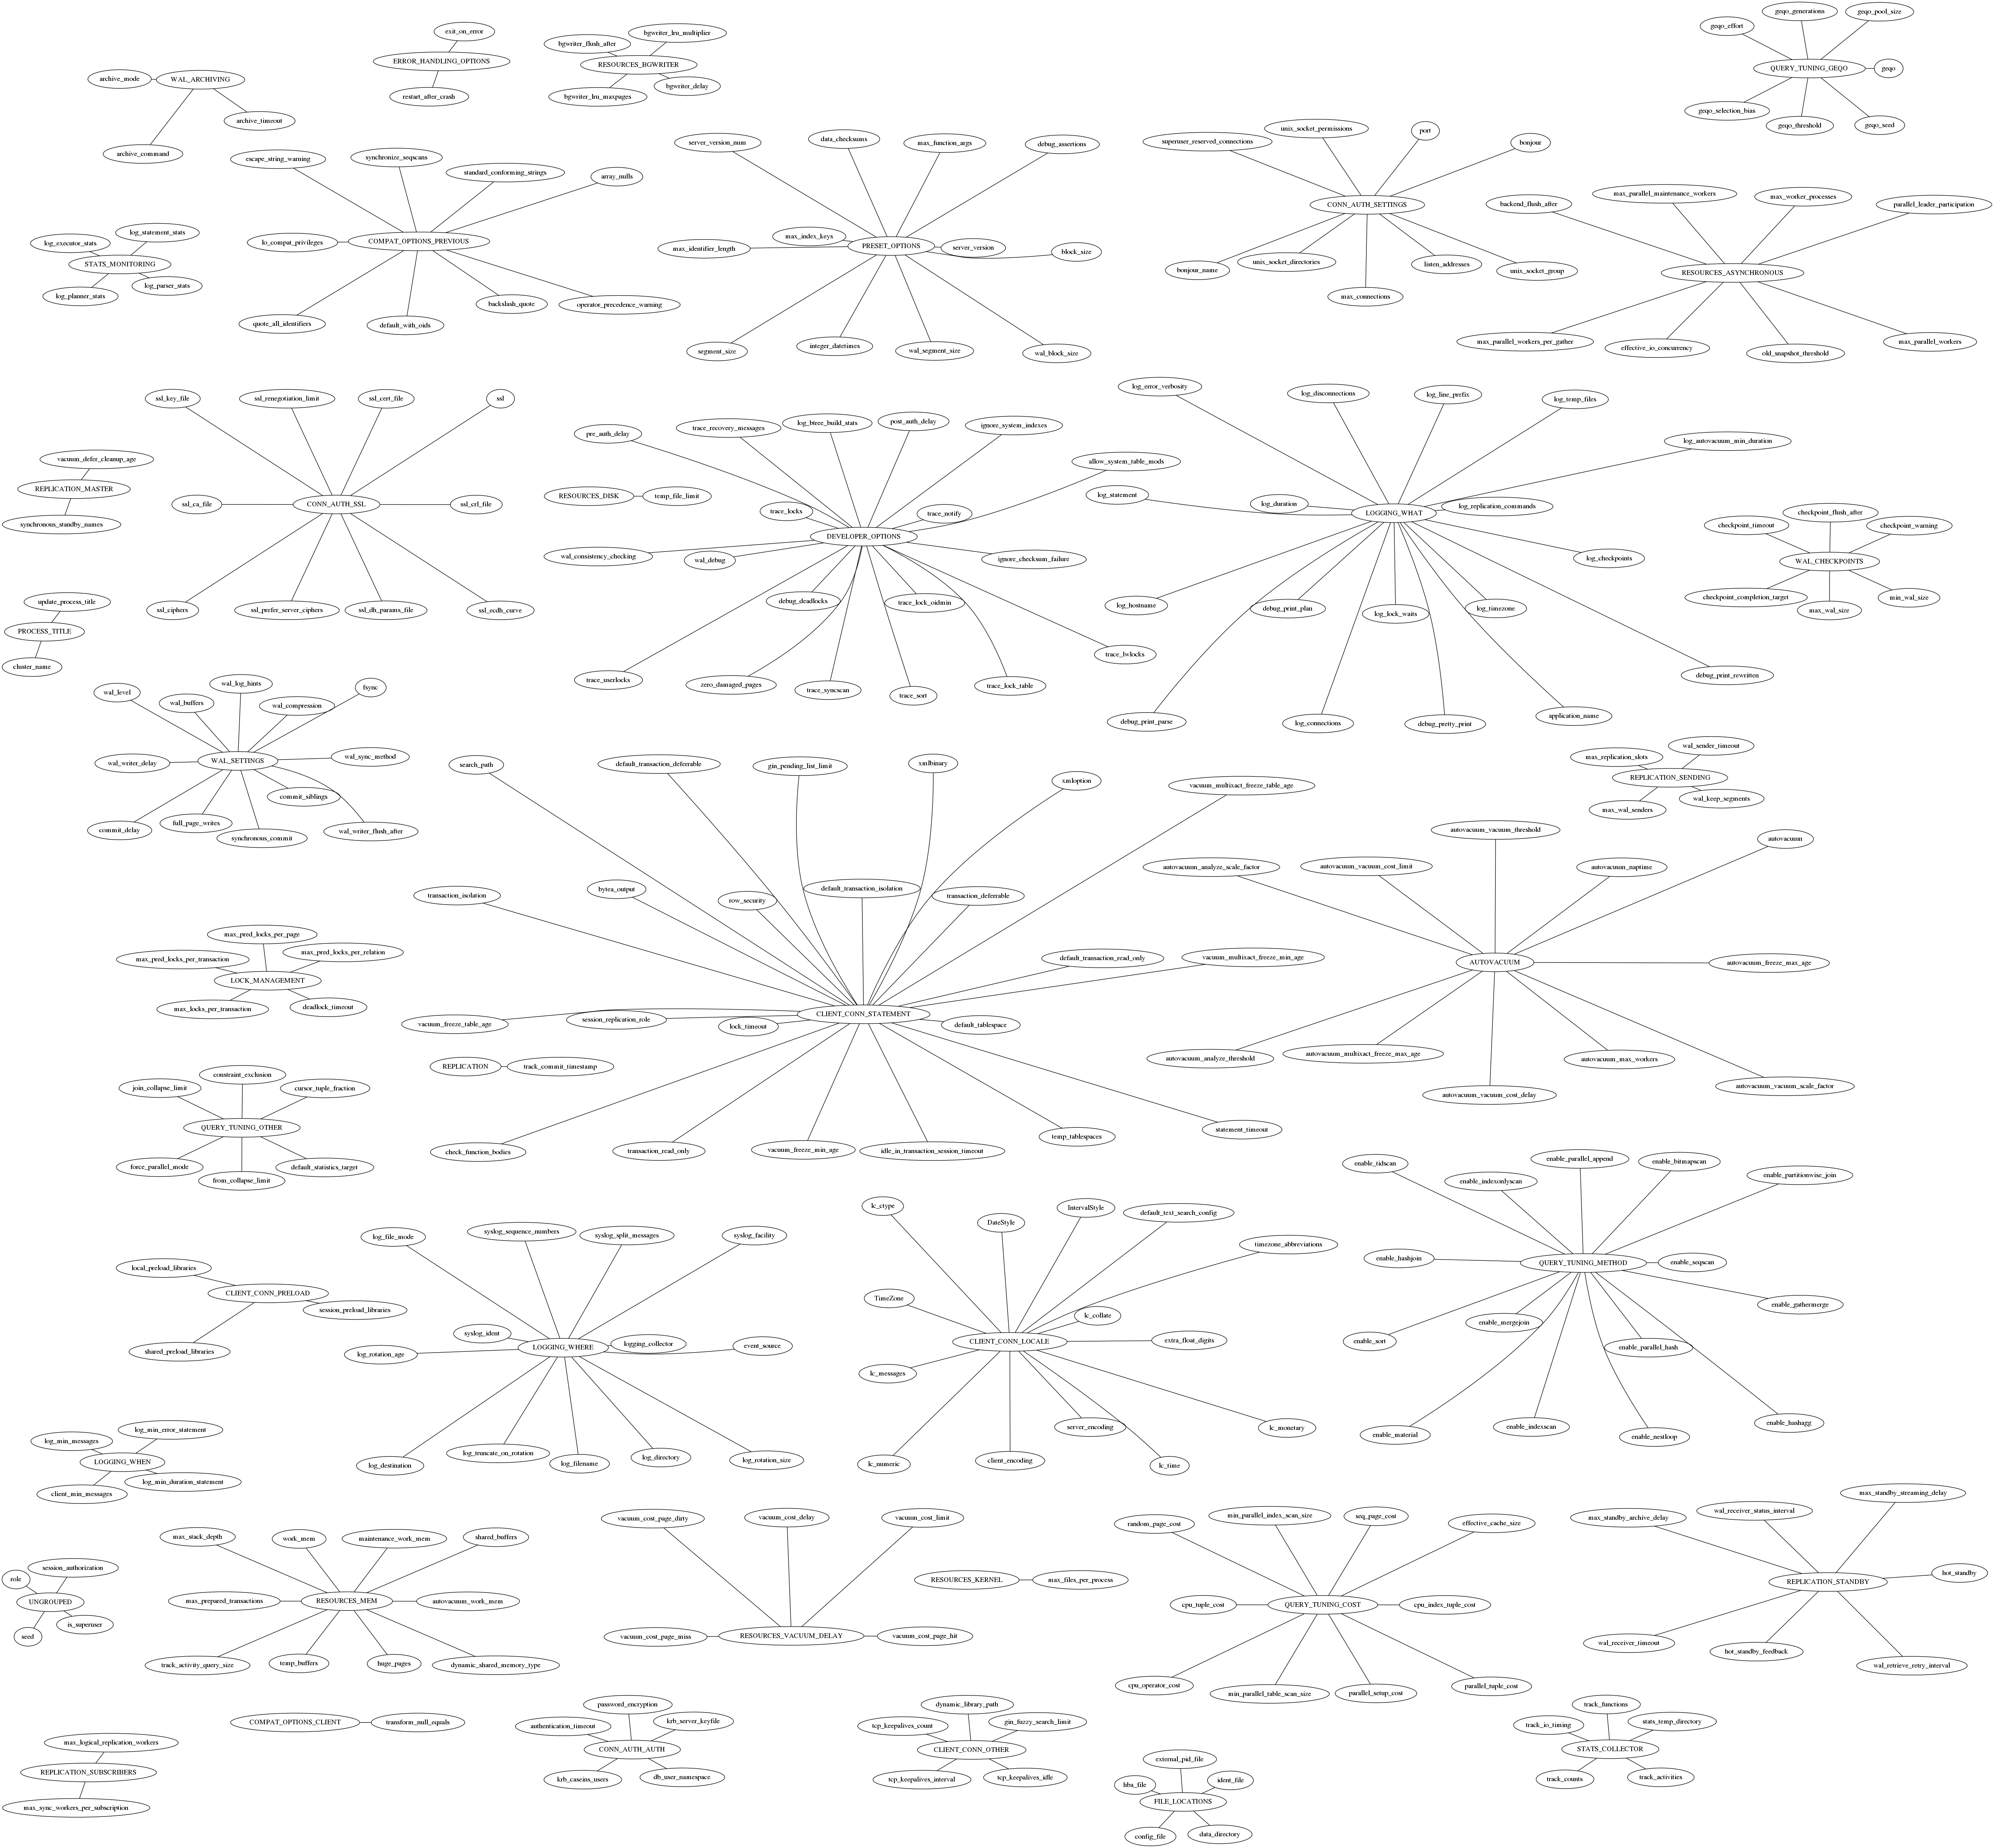
\includegraphics[width=0.75\textwidth,center]{pg_options.png}

    \end{center}
\end{frame}

\begin{frame}
    \frametitle{}
    \begin{center}

        \includegraphics[width=0.75\textwidth,center]{sysctl_small.jpg}

    \end{center}
\end{frame}

\fontsize{13pt}{14}\selectfont
\section{Execution scheduling}
\fontsize{17pt}{18}\selectfont

\begin{frame}[fragile]{}
    \frametitle{}
    \begin{center}

        \begin{minted}[fontsize=\normalsize]{bash}
            # Experiment 1
            transaction type: pg_long.sql
            latency average = 1312.903 ms

            # Experiment 2
            SQL script 1: pg_long.sql
             - weight: 1 (targets 50.0% of total)
             - latency average = 1426.928 ms

            SQL script 2: pg_short.sql
             - weight: 1 (targets 50.0% of total)
             - latency average = 303.092 ms
        \end{minted}

    \end{center}
\end{frame}

\begin{frame}
    \frametitle{}
    \begin{center}
        \textbf{Scheduling}

        \vspace{1.0cm}

        \only<1>{
            \begin{tikzpicture}
                \draw[
                    line width=0.5mm,
                    rounded corners=0.2cm,
                    dashed
                ] (0,0) rectangle (2,2) node[pos=.5] {};

                \draw[
                    line width=0.5mm,
                    rounded corners=0.2cm,
                    fill=red!30
                ] (0.25,0.25) rectangle (1.75,1.75) node[pos=.5] {\textbf{T1}};

                \draw[
                    line width=0.5mm,
                    rounded corners=0.1cm,
                    fill=red!30
                ] (2.25,0.25) rectangle (2.75,0.75) node[pos=.5] {\textbf{c}};

                \draw[
                    line width=0.5mm,
                    rounded corners=0.2cm,
                    dashed
                ] (4,0) rectangle (6,2) node[pos=.5] {};

                \draw[
                    line width=0.5mm,
                    rounded corners=0.2cm,
                    color=white
                ] (4.25,-1.25) rectangle (5.75,-2.75) node[pos=.5] {};

                \draw[
                    line width=0.5mm,
                    rounded corners=0.2cm,
                    fill=blue!30
                ] (4.25,0.25) rectangle (5.75,1.75) node[pos=.5] {\textbf{T2}};

                \draw[
                    line width=0.5mm,
                    rounded corners=0.1cm,
                    fill=blue!30
                ] (6.25,0.25) rectangle (6.75,0.75) node[pos=.5] {\textbf{c}};

            \end{tikzpicture}
        }

        \only<2>{
            \begin{tikzpicture}
                \draw[
                    line width=0.5mm,
                    rounded corners=0.2cm,
                    dashed
                ] (0,0) rectangle (2,2) node[pos=.5] {};

                \draw[
                    line width=0.5mm,
                    rounded corners=0.2cm,
                    fill=red!30
                ] (0.25,0.25) rectangle (1.75,1.75) node[pos=.5] {\textbf{T1}};

                \draw[
                    line width=0.5mm,
                    rounded corners=0.1cm,
                    fill=red!30
                ] (2.25,0.25) rectangle (2.75,0.75) node[pos=.5] {\textbf{c}};

                \draw[
                    line width=0.5mm,
                    rounded corners=0.2cm,
                    dashed
                ] (4,0) rectangle (6,2) node[pos=.5] {};

                \draw[
                    line width=0.5mm,
                    rounded corners=0.2cm,
                    fill=red!30
                ] (4.25,0.25) rectangle (5.75,1.75) node[pos=.5] {\textbf{T3}};

                \draw[
                    line width=0.5mm,
                    rounded corners=0.2cm,
                    fill=blue!30
                ] (4.25,-1.25) rectangle (5.75,-2.75) node[pos=.5] {\textbf{T2}};

                \draw[
                    line width=0.5mm,
                    rounded corners=0.1cm,
                    fill=blue!30
                ] (6.25,0.25) rectangle (6.75,0.75) node[pos=.5] {\textbf{c}};

            \end{tikzpicture}
        }

        \only<3>{
            \begin{tikzpicture}
                \draw[
                    line width=0.5mm,
                    rounded corners=0.2cm,
                    dashed
                ] (0,0) rectangle (2,2) node[pos=.5] {};

                \draw[
                    line width=0.5mm,
                    rounded corners=0.2cm,
                    fill=blue!30
                ] (0.25,0.25) rectangle (1.75,1.75) node[pos=.5] {\textbf{T2}};

                \draw[
                    line width=0.5mm,
                    rounded corners=0.1cm,
                    fill=red!30
                ] (2.25,0.25) rectangle (2.75,0.75) node[pos=.5] {\textbf{c}};

                \draw[
                    line width=0.5mm,
                    rounded corners=0.2cm,
                    dashed
                ] (4,0) rectangle (6,2) node[pos=.5] {};

                \draw[
                    line width=0.5mm,
                    rounded corners=0.2cm,
                    fill=red!30
                ] (4.25,0.25) rectangle (5.75,1.75) node[pos=.5] {\textbf{T3}};

                \draw[
                    line width=0.5mm,
                    rounded corners=0.2cm,
                    color=white
                ] (4.25,-1.25) rectangle (5.75,-2.75) node[pos=.5] {};

                \draw[
                    line width=0.5mm,
                    rounded corners=0.1cm,
                    fill=blue!30
                ] (6.25,0.25) rectangle (6.75,0.75) node[pos=.5] {\textbf{c}};

            \end{tikzpicture}
        }

        \only<4>{
            \begin{tikzpicture}
                \draw[
                    line width=0.5mm,
                    rounded corners=0.2cm,
                    dashed
                ] (0,0) rectangle (2,2) node[pos=.5] {};

                \draw[
                    line width=0.5mm,
                    rounded corners=0.2cm,
                    fill=blue!30
                ] (0.25,0.25) rectangle (1.75,1.75) node[pos=.5] {\textbf{T2}};

                \draw[
                    line width=0.5mm,
                    rounded corners=0.1cm,
                    fill=red!30
                ] (2.25,0.25) rectangle (2.75,0.75) node[pos=.5] {\textbf{c}};

                \draw[
                    <-,
                    line width=0.75mm,
                ] (2.5,0.25) to [controls=+(-90:2) and +(-90:2)]  (6.5,.5);

                \draw[
                    line width=0.5mm,
                    rounded corners=0.2cm,
                    dashed
                ] (4,0) rectangle (6,2) node[pos=.5] {};

                \draw[
                    line width=0.5mm,
                    rounded corners=0.2cm,
                    fill=red!30
                ] (4.25,0.25) rectangle (5.75,1.75) node[pos=.5] {\textbf{T3}};

                \draw[
                    line width=0.5mm,
                    rounded corners=0.2cm,
                    color=white
                ] (4.25,-1.25) rectangle (5.75,-2.75) node[pos=.5] {};

                \draw[
                    line width=0.5mm,
                    rounded corners=0.1cm,
                    fill=blue!30
                ] (6.25,0.25) rectangle (6.75,0.75) node[pos=.5] {\textbf{c}};

            \end{tikzpicture}
        }

    \end{center}
\end{frame}

\begin{frame}[fragile]{}
    \frametitle{}
    \begin{center}

        \begin{minted}[fontsize=\normalsize]{bash}
        # Experiment 1
        12,396,382,649      cache-misses # 28.562%
         2,750              cpu-migrations

        # Experiment 2
        20,665,817,234      cache-misses # 28.533%
        10,460              cpu-migrations
        \end{minted}

    \end{center}
\end{frame}

\begin{frame}
    \frametitle{}
    \begin{center}

        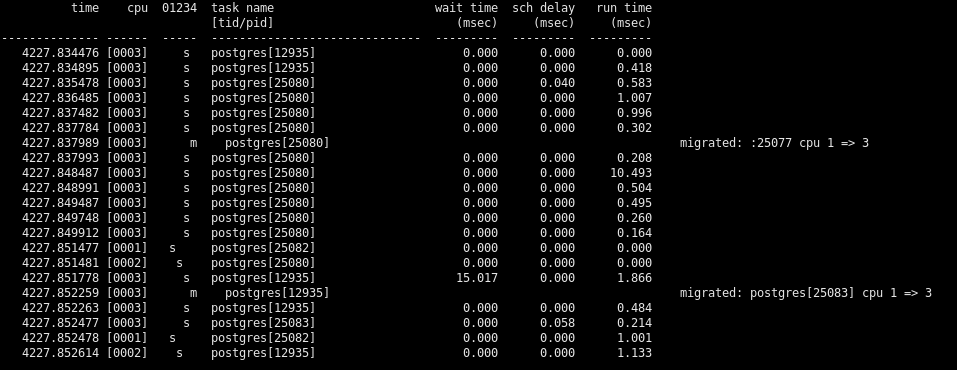
\includegraphics[width=1.0\textwidth,center]{migrations.png}

    \end{center}
\end{frame}

\begin{frame}
    \frametitle{}
    \begin{center}
    \textbf{Tunables}

        \begin{itemize}
            \item <+->
        \end{itemize}

        \begin{itemize}[label={\MVRightarrow}]
            \item <+-> /proc/sys/kernel/sched\_migration\_cost\_ns
            \item <+-> /proc/sys/kernel/sched\_min\_granularity\_ns
            \item <+-> schedule policy (BATCH / OTHER)
        \end{itemize}

    \end{center}
\end{frame}

\begin{frame}[fragile]{}
    \frametitle{}
    \begin{center}
    \textbf{pgbench and pg\_dump}

        \begin{minted}[fontsize=\normalsize]{bash}
            # Experiment 1
            SCHED_OTHER
            real    1m5.845s
            user    0m9.573s
            sys     0m3.475s

            # Experiment 2
            SCHED_BATCH and prioritized
            real    0m51.771s
            user    0m9.017s
            sys     0m2.967s
        \end{minted}

    \end{center}
\end{frame}

\begin{frame}
    \frametitle{}
    \begin{center}
    \textbf{HyperThreading}

        \begin{itemize}
            \item <+->
        \end{itemize}

        \begin{itemize}[label={\MVRightarrow}]
            \item <+-> Less deviation for latency
            \item <+-> Share execution state and cache
            \item <+-> Spin locks have significant impact
            \item <+-> PAUSE instruction (skylake latency 140)
        \end{itemize}

        \normalsize{Intel® 64 and IA-32 Architectures Optimization Reference Manual}
    \end{center}
\end{frame}

\begin{frame}
    \frametitle{}
    \begin{center}
    \textbf{Latency rolling standard deviation}

        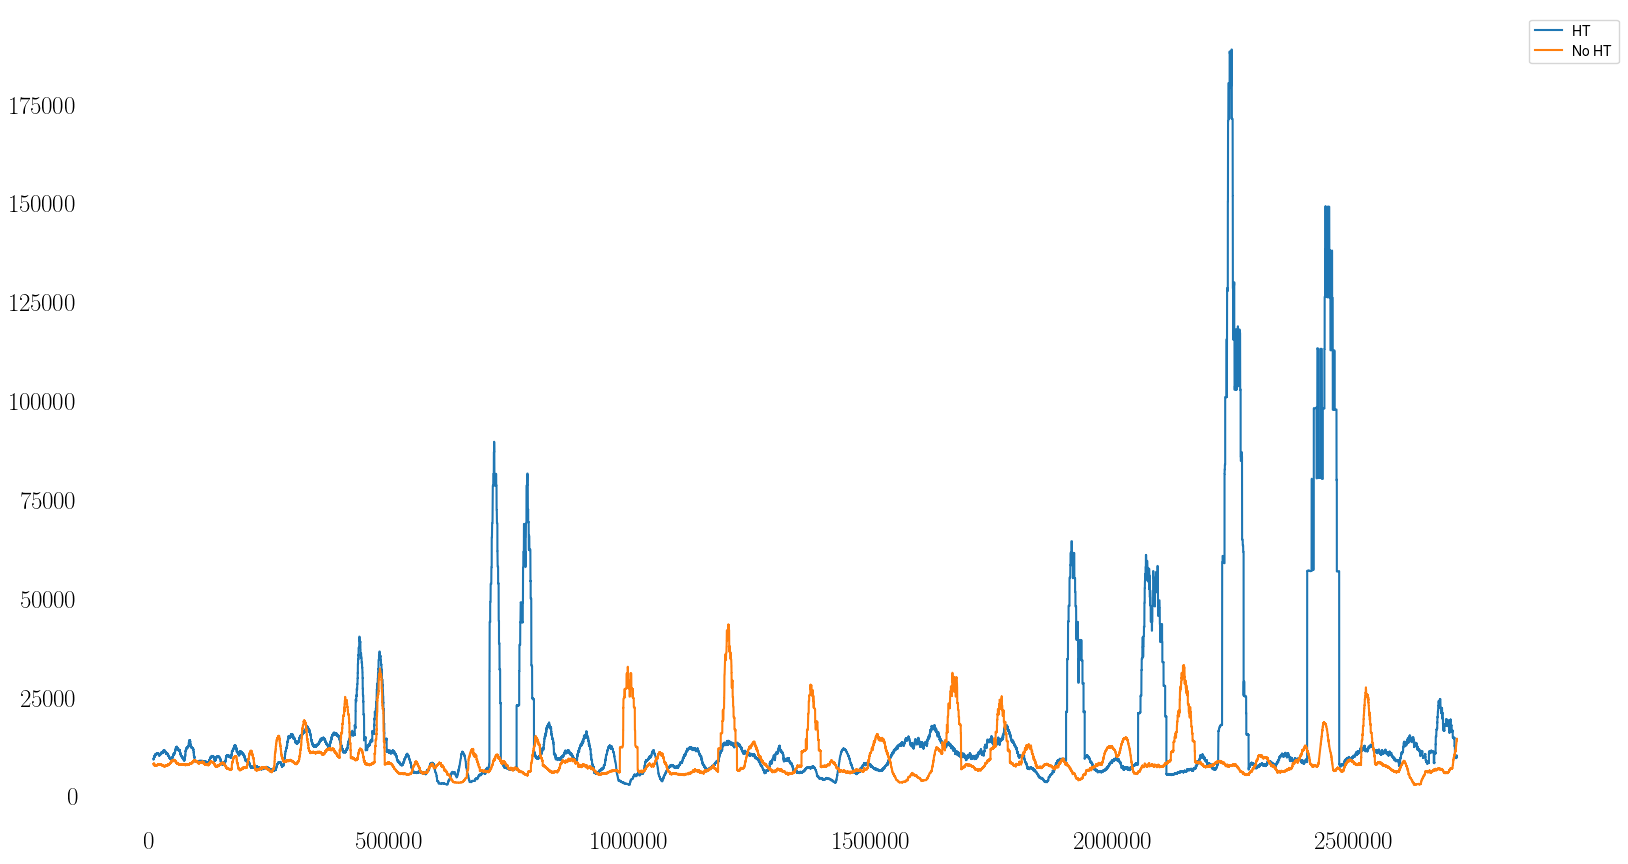
\includegraphics[width=0.9\textwidth,center]{hyperthreading.png}

    \end{center}
\end{frame}

\begin{frame}
    \frametitle{}
    \begin{center}
    \textbf{Latency rolling standard deviation, readonly}

        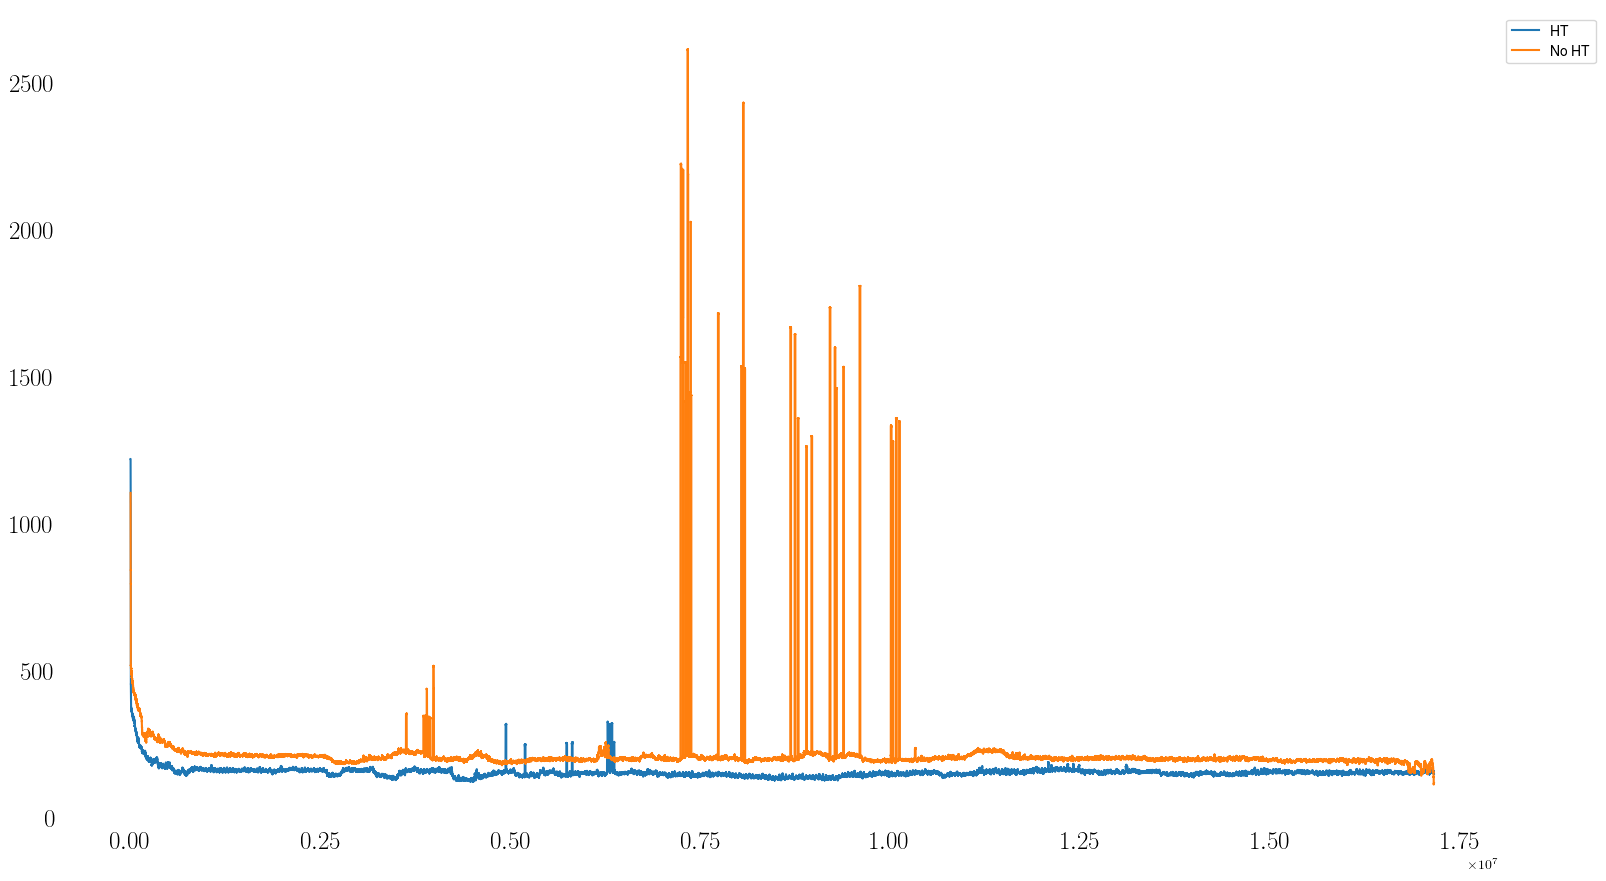
\includegraphics[width=0.9\textwidth,center]{hyperthreading_readonly.png}

    \end{center}
\end{frame}

\fontsize{13pt}{14}\selectfont
\section{Virtualization?}
\fontsize{17pt}{18}\selectfont

\begin{frame}
    \frametitle{}
    \begin{center}
    \textbf{Timekeeping}

        \begin{itemize}
            \item <+->
        \end{itemize}

        \begin{itemize}[label={\MVRightarrow}]
            \item <+-> Statistical sampling \\ (occasional incorrect charging)
            \item <+-> Exact measurement (TSC time drift)
            \item <+-> /sys/devices/system/clocksource/clocksource0/
        \end{itemize}

        \normalsize{Timekeeping in VMware Virtual: Information Guide}
    \end{center}
\end{frame}

\begin{frame}
    \frametitle{}
    \begin{center}
        \textbf{Scheduling}

        \vspace{1.0cm}

        \only<1>{
            \begin{tikzpicture}
                \draw[
                    line width=0.3mm,
                    pattern=north west lines,
                    pattern color=blue!30
                    ] (0,3) rectangle (1,3.3) node[pos=.5] {};

                \draw[
                    line width=0.5mm,
                    rounded corners=0.2cm,
                    fill=blue!30
                    ] (0,-1) rectangle (6,-2) node[pos=.5] {\textbf{Hypervisor}};

                \draw[
                    <-,
                    line width=0.75mm,
                ] (1,1) to (3,-1);

                \draw[
                    line width=0.5mm,
                    rounded corners=0.2cm,
                    dashed
                ] (0,0) rectangle (2,2) node[pos=.5] {};

                \draw[
                    line width=0.5mm,
                    rounded corners=0.2cm,
                    fill=red!30
                ] (0.25,0.25) rectangle (1.75,1.75) node[pos=.5] {\textbf{VM1}};

                \draw[
                    line width=0.5mm,
                    rounded corners=0.2cm,
                    fill=gray!30
                ] (4.25,0.25) rectangle (5.75,1.75) node[pos=.5] {\textbf{VM2}};

            \end{tikzpicture}
        }

        \only<2>{
            \begin{tikzpicture}
                \draw[
                    line width=0.3mm,
                    pattern=north west lines,
                    pattern color=blue!30
                    ] (0,3) rectangle (2,3.3) node[pos=.5] {};

                \draw[
                    line width=0.3mm,
                    pattern=north west lines,
                    pattern color=gray!30,
                    dashed
                    ] (2,3) rectangle (4,3.3) node[pos=.5] {};

                \draw[
                    line width=0.5mm,
                    rounded corners=0.2cm,
                    fill=blue!30
                    ] (0,-1) rectangle (6,-2) node[pos=.5] {\textbf{Hypervisor}};

                \draw[
                    <-,
                    line width=0.75mm,
                ] (5,1) to (3,-1);

                \draw[
                    line width=0.5mm,
                    rounded corners=0.2cm,
                    fill=gray!30
                ] (0.25,0.25) rectangle (1.75,1.75) node[pos=.5] {\textbf{VM1}};

                \draw[
                    line width=0.5mm,
                    rounded corners=0.2cm,
                    dashed
                ] (4,0) rectangle (6,2) node[pos=.5] {};

                \draw[
                    line width=0.5mm,
                    rounded corners=0.2cm,
                    fill=red!30
                ] (4.25,0.25) rectangle (5.75,1.75) node[pos=.5] {\textbf{VM2}};

            \end{tikzpicture}
        }

        \only<3>{
            \begin{tikzpicture}
                \draw[
                    line width=0.3mm,
                    pattern=north west lines,
                    pattern color=blue!30
                    ] (0,3) rectangle (2,3.3) node[pos=.5] {};

                \draw[
                    line width=0.3mm,
                    pattern=north west lines,
                    pattern color=gray!30,
                    dashed
                    ] (2,3) rectangle (4,3.3) node[pos=.5] {};

                \draw[
                    line width=0.3mm,
                    pattern=north west lines,
                    pattern color=blue!30
                    ] (4,3) rectangle (6,3.3) node[pos=.5] {};

                \draw[
                    line width=0.5mm,
                    rounded corners=0.2cm,
                    fill=blue!30
                    ] (0,-1) rectangle (6,-2) node[pos=.5] {\textbf{Hypervisor}};

                \draw[
                    <-,
                    line width=0.75mm,
                ] (1,1) to (3,-1);

                \draw[
                    line width=0.5mm,
                    rounded corners=0.2cm,
                    dashed
                ] (0,0) rectangle (2,2) node[pos=.5] {};

                \draw[
                    line width=0.5mm,
                    rounded corners=0.2cm,
                    fill=red!30
                ] (0.25,0.25) rectangle (1.75,1.75) node[pos=.5] {\textbf{VM1}};

                \draw[
                    line width=0.5mm,
                    rounded corners=0.2cm,
                    fill=gray!30
                ] (4.25,0.25) rectangle (5.75,1.75) node[pos=.5] {\textbf{VM2}};

            \end{tikzpicture}
        }

    \end{center}
\end{frame}

\begin{frame}
    \frametitle{}
    \begin{center}
    \textbf{vDSO}

        \begin{itemize}[label={\MVRightarrow}]
            \item gettimeofday
            \item clock\_gettime
            \item XEN doesn't support vDSO for them
            \item unnecessary context switches to a kernel
        \end{itemize}

        \normalsize{\href{
            https://blog.packagecloud.io/eng/2017/03/08/system-calls-are-much-slower-on-ec2/
        }{Two frequently used system calls are ~77\% slower on AWS EC2}}
    \end{center}
\end{frame}

\begin{frame}
    \frametitle{}
    \begin{center}
    \textbf{Latency m4.xlarge XEN/TSC}

        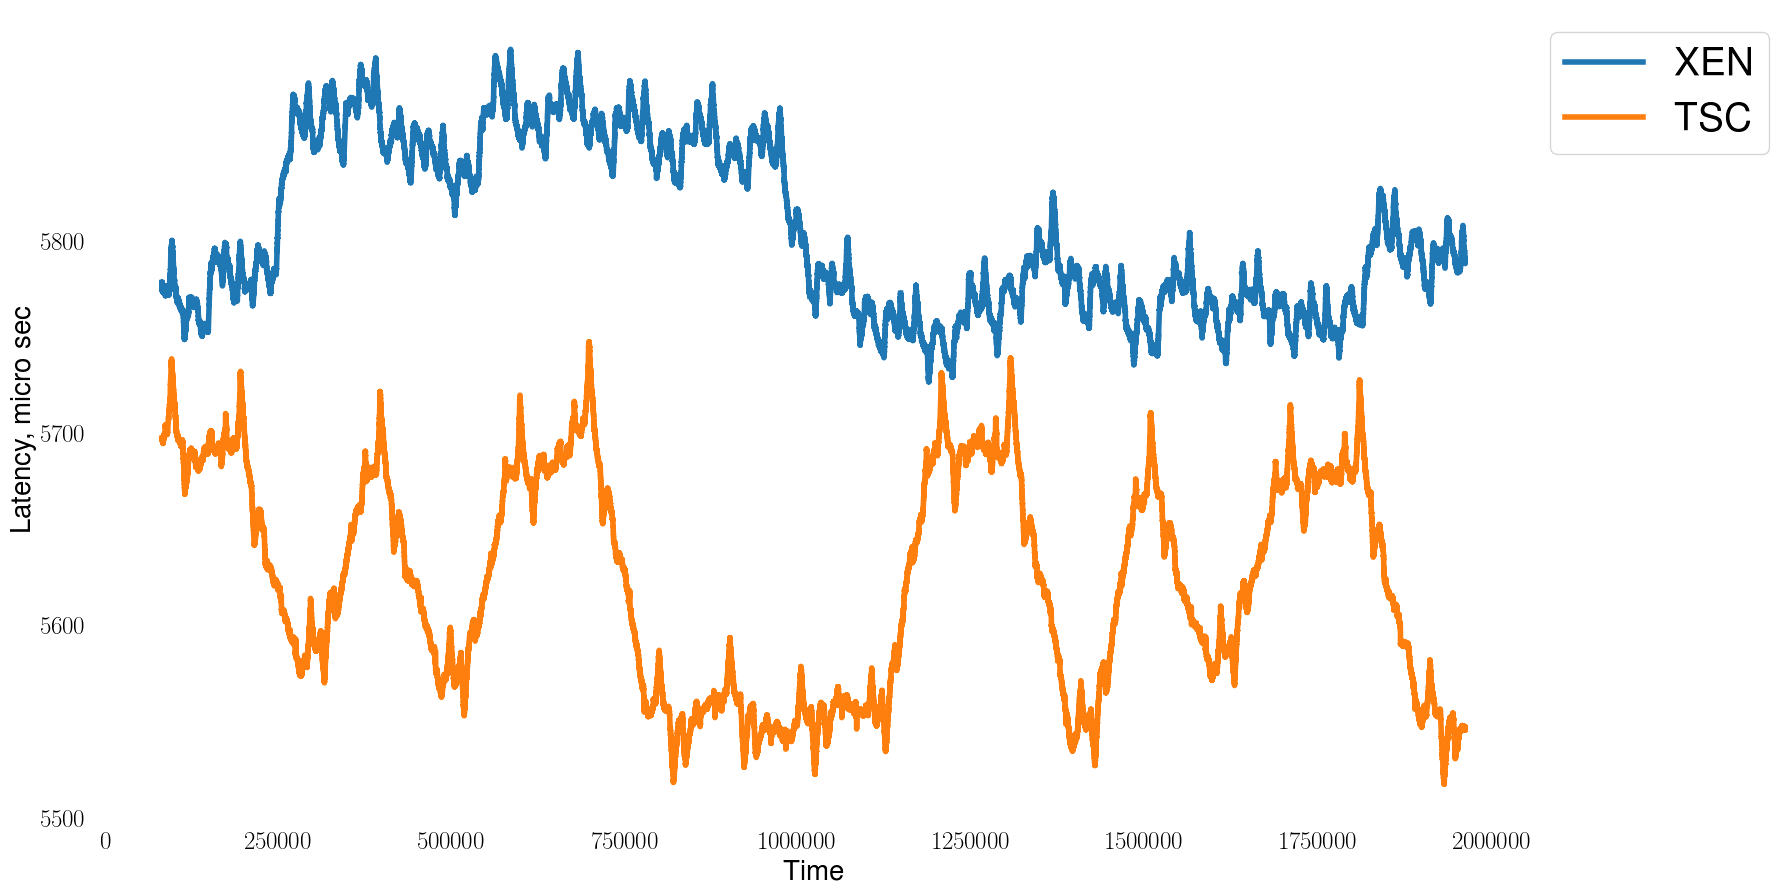
\includegraphics[width=0.9\textwidth,center]{m4_clock_source.png}

    \end{center}
\end{frame}

\begin{frame}
    \frametitle{}
    \begin{center}
    \textbf{Latency m5.xlarge KVM-CLOCK/TSC}

        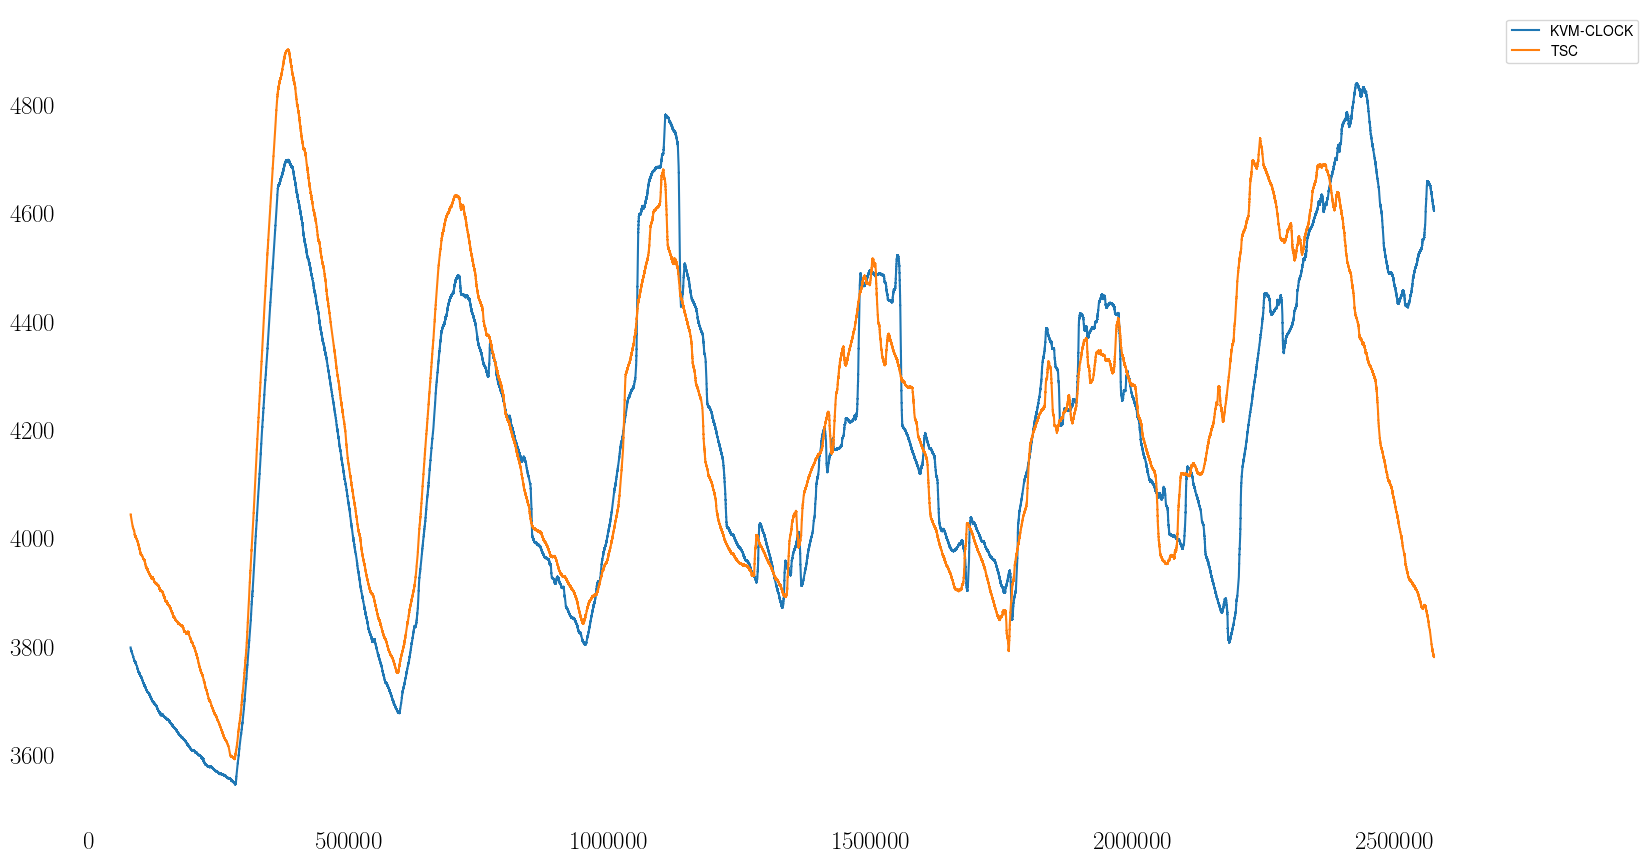
\includegraphics[width=0.9\textwidth,center]{m5_clock_source.png}

    \end{center}
\end{frame}

\fontsize{13pt}{14}\selectfont
\section{Memory}
\fontsize{17pt}{18}\selectfont

\begin{frame}
    \frametitle{}
    \begin{center}
        \textbf{Dirty pages}

        \vspace{1.0cm}

        \only<1>{
            \begin{tikzpicture}
                \draw[
                    line width=0.5mm,
                    rounded corners=0.2cm,
                    pattern=north west lines,
                    pattern color=blue!30
                    ] (0,-1) rectangle (6,-2) node[pos=.5] {\textbf{OS Cache}};

                \draw[
                    line width=0.5mm,
                    rounded corners=0.2cm,
                    pattern=north west lines,
                    pattern color=green!30
                    ] (0,-2.25) rectangle (6,-3.25) node[pos=.5] {\textbf{Storage}};

                \draw[
                    line width=0.5mm,
                    rounded corners=0.2cm,
                    fill=blue!30
                    ] (-3,2.75) rectangle (0,1.75) node[pos=.5] {\textbf{bgw}};

                \draw[
                    line width=0.5mm,
                    rounded corners=0.2cm,
                    color=white
                    ] (-3.1,2.85) rectangle (0.1,1.65) node[pos=.5] {};

                \draw[
                    line width=0.5mm,
                    rounded corners=0.2cm,
                    fill=blue!30
                    ] (-3,1.5) rectangle (0,0.5) node[pos=.5] {\textbf{linux}};

                \draw[
                    line width=0.5mm,
                    rounded corners=0.2cm,
                    fill=blue!30
                    ] (-3,0.25) rectangle (0,-0.75) node[pos=.5] {\textbf{chkp}};

                \draw[
                    line width=0.5mm,
                    rounded corners=0.1cm,
                    fill=red!30
                ] (1.25,2.25) rectangle (1.75,2.75) node[pos=.5] {};

                \draw[
                    line width=0.5mm,
                    rounded corners=0.1cm,
                    fill=gray!30
                ] (4.25,2.25) rectangle (4.75,2.75) node[pos=.5] {};

                \draw[
                    line width=0.5mm,
                    rounded corners=0.1cm,
                    fill=gray!30
                ] (3.25,2.25) rectangle (3.75,2.75) node[pos=.5] {};

                \draw[
                    line width=0.5mm,
                    rounded corners=0.1cm,
                    fill=gray!30
                ] (2.25,2.25) rectangle (2.75,2.75) node[pos=.5] {};

                \draw[
                    line width=0.5mm,
                    rounded corners=0.1cm,
                    fill=gray!30
                ] (1.25,1.25) rectangle (1.75,1.75) node[pos=.5] {};

                \draw[
                    line width=0.5mm,
                    rounded corners=0.1cm,
                    fill=red!30
                ] (4.25,1.25) rectangle (4.75,1.75) node[pos=.5] {};

                \draw[
                    line width=0.5mm,
                    rounded corners=0.1cm,
                    fill=gray!30
                ] (3.25,1.25) rectangle (3.75,1.75) node[pos=.5] {};

                \draw[
                    line width=0.5mm,
                    rounded corners=0.1cm,
                    fill=gray!30
                ] (2.25,1.25) rectangle (2.75,1.75) node[pos=.5] {};

                \draw[
                    line width=0.5mm,
                    rounded corners=0.1cm,
                    fill=gray!30
                ] (1.25,0.25) rectangle (1.75,0.75) node[pos=.5] {};

                \draw[
                    line width=0.5mm,
                    rounded corners=0.1cm,
                    fill=gray!30
                ] (4.25,0.25) rectangle (4.75,0.75) node[pos=.5] {};

                \draw[
                    line width=0.5mm,
                    rounded corners=0.1cm,
                    fill=red!30
                ] (3.25,0.25) rectangle (3.75,0.75) node[pos=.5] {};

                \draw[
                    line width=0.5mm,
                    rounded corners=0.1cm,
                    fill=gray!30
                ] (2.25,0.25) rectangle (2.75,0.75) node[pos=.5] {};
            \end{tikzpicture}
        }

        \only<2>{
            \begin{tikzpicture}
                \draw[
                    line width=0.5mm,
                    rounded corners=0.2cm,
                    pattern=north west lines,
                    pattern color=blue!30
                    ] (0,-1) rectangle (6,-2) node[pos=.5] {\textbf{OS Cache}};

                \draw[
                    line width=0.5mm,
                    rounded corners=0.2cm,
                    pattern=north west lines,
                    pattern color=green!30
                    ] (0,-2.25) rectangle (6,-3.25) node[pos=.5] {\textbf{Storage}};

                \draw[
                    line width=0.5mm,
                    rounded corners=0.2cm,
                    fill=blue!30
                    ] (-3,2.75) rectangle (0,1.75) node[pos=.5] {\textbf{bgw}};

                \draw[
                    line width=0.5mm,
                    rounded corners=0.2cm,
                    dashed
                    ] (-3.1,2.85) rectangle (0.1,1.65) node[pos=.5] {};

                \draw[
                    line width=0.5mm,
                    rounded corners=0.2cm,
                    fill=blue!30
                    ] (-3,1.5) rectangle (0,0.5) node[pos=.5] {\textbf{linux}};

                \draw[
                    line width=0.5mm,
                    rounded corners=0.2cm,
                    fill=blue!30
                    ] (-3,0.25) rectangle (0,-0.75) node[pos=.5] {\textbf{chkp}};

                \draw[
                    line width=0.5mm,
                    rounded corners=0.1cm,
                    fill=red!30
                ] (1.25,2.25) rectangle (1.75,2.75) node[pos=.5] {};

                \draw[
                    line width=0.5mm,
                    rounded corners=0.1cm,
                    fill=gray!30
                ] (4.25,2.25) rectangle (4.75,2.75) node[pos=.5] {};

                \draw[
                    line width=0.5mm,
                    rounded corners=0.1cm,
                    fill=gray!30
                ] (3.25,2.25) rectangle (3.75,2.75) node[pos=.5] {};

                \draw[
                    line width=0.5mm,
                    rounded corners=0.1cm,
                    fill=gray!30
                ] (2.25,2.25) rectangle (2.75,2.75) node[pos=.5] {};

                \draw[
                    line width=0.5mm,
                    rounded corners=0.1cm,
                    fill=gray!30
                ] (1.25,1.25) rectangle (1.75,1.75) node[pos=.5] {};

                \draw[
                    line width=0.5mm,
                    rounded corners=0.1cm,
                    fill=red!30
                ] (4.25,1.25) rectangle (4.75,1.75) node[pos=.5] {};

                \draw[
                    line width=0.5mm,
                    rounded corners=0.1cm,
                    fill=gray!30
                ] (3.25,1.25) rectangle (3.75,1.75) node[pos=.5] {};

                \draw[
                    line width=0.5mm,
                    rounded corners=0.1cm,
                    fill=gray!30
                ] (2.25,1.25) rectangle (2.75,1.75) node[pos=.5] {};

                \draw[
                    line width=0.5mm,
                    rounded corners=0.1cm,
                    fill=gray!30
                ] (1.25,0.25) rectangle (1.75,0.75) node[pos=.5] {};

                \draw[
                    line width=0.5mm,
                    rounded corners=0.1cm,
                    fill=gray!30
                ] (4.25,0.25) rectangle (4.75,0.75) node[pos=.5] {};

                \draw[
                    line width=0.5mm,
                    rounded corners=0.1cm,
                    fill=gray!30
                ] (3.25,0.25) rectangle (3.75,0.75) node[pos=.5] {};

                \draw[
                    line width=0.5mm,
                    rounded corners=0.1cm,
                    fill=gray!30
                ] (2.25,0.25) rectangle (2.75,0.75) node[pos=.5] {};

                \draw[
                    line width=0.5mm,
                    rounded corners=0.1cm,
                    fill=red!30
                ] (3.25,-1.25) rectangle (3.75,-1.75) node[pos=.5] {};

                \draw[
                    ->,
                    line width=0.75mm,
                ] (3.5,0.25) to (3.5,-1.25);

             \end{tikzpicture}
        }

        \only<3>{
            \begin{tikzpicture}
                \draw[
                    line width=0.5mm,
                    rounded corners=0.2cm,
                    pattern=north west lines,
                    pattern color=blue!30
                    ] (0,-1) rectangle (6,-2) node[pos=.5] {\textbf{OS Cache}};

                \draw[
                    line width=0.5mm,
                    rounded corners=0.2cm,
                    pattern=north west lines,
                    pattern color=green!30
                    ] (0,-2.25) rectangle (6,-3.25) node[pos=.5] {\textbf{Storage}};

                \draw[
                    line width=0.5mm,
                    rounded corners=0.2cm,
                    fill=blue!30
                    ] (-3,2.75) rectangle (0,1.75) node[pos=.5] {\textbf{bgw}};

                \draw[
                    line width=0.5mm,
                    rounded corners=0.2cm,
                    color=white
                    ] (-3.1,2.85) rectangle (0.1,1.65) node[pos=.5] {};

                \draw[
                    line width=0.5mm,
                    rounded corners=0.2cm,
                    fill=blue!30
                    ] (-3,1.5) rectangle (0,0.5) node[pos=.5] {\textbf{linux}};

                \draw[
                    line width=0.5mm,
                    rounded corners=0.2cm,
                    dashed
                    ] (-3.1,1.6) rectangle (0.1,0.4) node[pos=.5] {};

                \draw[
                    line width=0.5mm,
                    rounded corners=0.2cm,
                    fill=blue!30
                    ] (-3,0.25) rectangle (0,-0.75) node[pos=.5] {\textbf{chkp}};

                \draw[
                    line width=0.5mm,
                    rounded corners=0.1cm,
                    fill=red!30
                ] (1.25,2.25) rectangle (1.75,2.75) node[pos=.5] {};

                \draw[
                    line width=0.5mm,
                    rounded corners=0.1cm,
                    fill=gray!30
                ] (4.25,2.25) rectangle (4.75,2.75) node[pos=.5] {};

                \draw[
                    line width=0.5mm,
                    rounded corners=0.1cm,
                    fill=gray!30
                ] (3.25,2.25) rectangle (3.75,2.75) node[pos=.5] {};

                \draw[
                    line width=0.5mm,
                    rounded corners=0.1cm,
                    fill=gray!30
                ] (2.25,2.25) rectangle (2.75,2.75) node[pos=.5] {};

                \draw[
                    line width=0.5mm,
                    rounded corners=0.1cm,
                    fill=gray!30
                ] (1.25,1.25) rectangle (1.75,1.75) node[pos=.5] {};

                \draw[
                    line width=0.5mm,
                    rounded corners=0.1cm,
                    fill=red!30
                ] (4.25,1.25) rectangle (4.75,1.75) node[pos=.5] {};

                \draw[
                    line width=0.5mm,
                    rounded corners=0.1cm,
                    fill=gray!30
                ] (3.25,1.25) rectangle (3.75,1.75) node[pos=.5] {};

                \draw[
                    line width=0.5mm,
                    rounded corners=0.1cm,
                    fill=gray!30
                ] (2.25,1.25) rectangle (2.75,1.75) node[pos=.5] {};

                \draw[
                    line width=0.5mm,
                    rounded corners=0.1cm,
                    fill=gray!30
                ] (1.25,0.25) rectangle (1.75,0.75) node[pos=.5] {};

                \draw[
                    line width=0.5mm,
                    rounded corners=0.1cm,
                    fill=gray!30
                ] (4.25,0.25) rectangle (4.75,0.75) node[pos=.5] {};

                \draw[
                    line width=0.5mm,
                    rounded corners=0.1cm,
                    fill=gray!30
                ] (3.25,0.25) rectangle (3.75,0.75) node[pos=.5] {};

                \draw[
                    line width=0.5mm,
                    rounded corners=0.1cm,
                    fill=gray!30
                ] (2.25,0.25) rectangle (2.75,0.75) node[pos=.5] {};

                \draw[
                    line width=0.5mm,
                    rounded corners=0.1cm,
                    fill=gray!30
                ] (3.25,-1.25) rectangle (3.75,-1.75) node[pos=.5] {};

                \draw[
                    line width=0.5mm,
                    rounded corners=0.1cm,
                    fill=red!30
                ] (3.25,-2.5) rectangle (3.75,-3) node[pos=.5] {};

                \draw[
                    ->,
                    line width=0.75mm,
                ] (3.5,-1.75) to (3.5,-2.5);

            \end{tikzpicture}
        }

        \only<4>{
            \begin{tikzpicture}
                \draw[
                    line width=0.5mm,
                    rounded corners=0.2cm,
                    pattern=north west lines,
                    pattern color=blue!30
                    ] (0,-1) rectangle (6,-2) node[pos=.5] {\textbf{OS Cache}};

                \draw[
                    line width=0.5mm,
                    rounded corners=0.2cm,
                    pattern=north west lines,
                    pattern color=green!30
                    ] (0,-2.25) rectangle (6,-3.25) node[pos=.5] {\textbf{Storage}};

                \draw[
                    line width=0.5mm,
                    rounded corners=0.2cm,
                    fill=blue!30
                    ] (-3,2.75) rectangle (0,1.75) node[pos=.5] {\textbf{bgw}};

                \draw[
                    line width=0.5mm,
                    rounded corners=0.2cm,
                    color=white
                    ] (-3.1,2.85) rectangle (0.1,1.65) node[pos=.5] {};

                \draw[
                    line width=0.5mm,
                    rounded corners=0.2cm,
                    fill=blue!30
                    ] (-3,1.5) rectangle (0,0.5) node[pos=.5] {\textbf{linux}};

                \draw[
                    line width=0.5mm,
                    rounded corners=0.2cm,
                    fill=blue!30
                    ] (-3,0.25) rectangle (0,-0.75) node[pos=.5] {\textbf{chkp}};

                \draw[
                    line width=0.5mm,
                    rounded corners=0.2cm,
                    dashed
                    ] (-3.1,0.35) rectangle (0.1,-0.85) node[pos=.5] {};

                \draw[
                    line width=0.5mm,
                    rounded corners=0.1cm,
                    fill=gray!30
                ] (1.25,2.25) rectangle (1.75,2.75) node[pos=.5] {};

                \draw[
                    line width=0.5mm,
                    rounded corners=0.1cm,
                    fill=gray!30
                ] (4.25,2.25) rectangle (4.75,2.75) node[pos=.5] {};

                \draw[
                    line width=0.5mm,
                    rounded corners=0.1cm,
                    fill=gray!30
                ] (3.25,2.25) rectangle (3.75,2.75) node[pos=.5] {};

                \draw[
                    line width=0.5mm,
                    rounded corners=0.1cm,
                    fill=gray!30
                ] (2.25,2.25) rectangle (2.75,2.75) node[pos=.5] {};

                \draw[
                    line width=0.5mm,
                    rounded corners=0.1cm,
                    fill=gray!30
                ] (1.25,1.25) rectangle (1.75,1.75) node[pos=.5] {};

                \draw[
                    line width=0.5mm,
                    rounded corners=0.1cm,
                    fill=gray!30
                ] (4.25,1.25) rectangle (4.75,1.75) node[pos=.5] {};

                \draw[
                    line width=0.5mm,
                    rounded corners=0.1cm,
                    fill=gray!30
                ] (3.25,1.25) rectangle (3.75,1.75) node[pos=.5] {};

                \draw[
                    line width=0.5mm,
                    rounded corners=0.1cm,
                    fill=gray!30
                ] (2.25,1.25) rectangle (2.75,1.75) node[pos=.5] {};

                \draw[
                    line width=0.5mm,
                    rounded corners=0.1cm,
                    fill=gray!30
                ] (1.25,0.25) rectangle (1.75,0.75) node[pos=.5] {};

                \draw[
                    line width=0.5mm,
                    rounded corners=0.1cm,
                    fill=gray!30
                ] (4.25,0.25) rectangle (4.75,0.75) node[pos=.5] {};

                \draw[
                    line width=0.5mm,
                    rounded corners=0.1cm,
                    fill=gray!30
                ] (3.25,0.25) rectangle (3.75,0.75) node[pos=.5] {};

                \draw[
                    line width=0.5mm,
                    rounded corners=0.1cm,
                    fill=gray!30
                ] (2.25,0.25) rectangle (2.75,0.75) node[pos=.5] {};

                \draw[
                    line width=0.5mm,
                    rounded corners=0.1cm,
                    fill=gray!30
                ] (4.25,-1.25) rectangle (4.75,-1.75) node[pos=.5] {};

                \draw[
                    line width=0.5mm,
                    rounded corners=0.1cm,
                    fill=red!30
                ] (4.25,-2.5) rectangle (4.75,-3) node[pos=.5] {};

                \draw[
                    line width=0.5mm,
                    rounded corners=0.1cm,
                    fill=gray!30
                ] (1.25,-1.25) rectangle (1.75,-1.75) node[pos=.5] {};

                \draw[
                    line width=0.5mm,
                    rounded corners=0.1cm,
                    fill=red!30
                ] (1.25,-2.5) rectangle (1.75,-3) node[pos=.5] {};

                \draw[
                    line width=0.5mm,
                    rounded corners=0.1cm,
                    fill=gray!30
                ] (3.25,-1.25) rectangle (3.75,-1.75) node[pos=.5] {};

                \draw[
                    line width=0.5mm,
                    rounded corners=0.1cm,
                    fill=red!30
                ] (3.25,-2.5) rectangle (3.75,-3) node[pos=.5] {};

                \draw[
                    ->,
                    line width=0.75mm,
                ] (1.5,2.25) to (1.5,-1.25);

                \draw[
                    ->,
                    line width=0.75mm,
                ] (4.5,2.25) to (4.5,-1.25);

                \draw[
                    ->,
                    line width=0.75mm,
                ] (1.5,-1.75) to (1.5,-2.5);

                \draw[
                    ->,
                    line width=0.75mm,
                ] (4.5,-1.75) to (4.5,-2.5);

            \end{tikzpicture}
        }

    \end{center}
\end{frame}

\begin{frame}
    \frametitle{}
    \begin{center}
    \textbf{Dirty pages}

        \begin{itemize}[label={\MVRightarrow}]
            \item vm.dirty\_ratio
            \item vm.dirty\_background\_ratio
            \item vm.dirty\_bytes
            \item vm.dirty\_backround\_bytes
        \end{itemize}

    \end{center}
\end{frame}

\begin{frame}
    \frametitle{}
    \begin{center}
    \textbf{Dirty pages}

    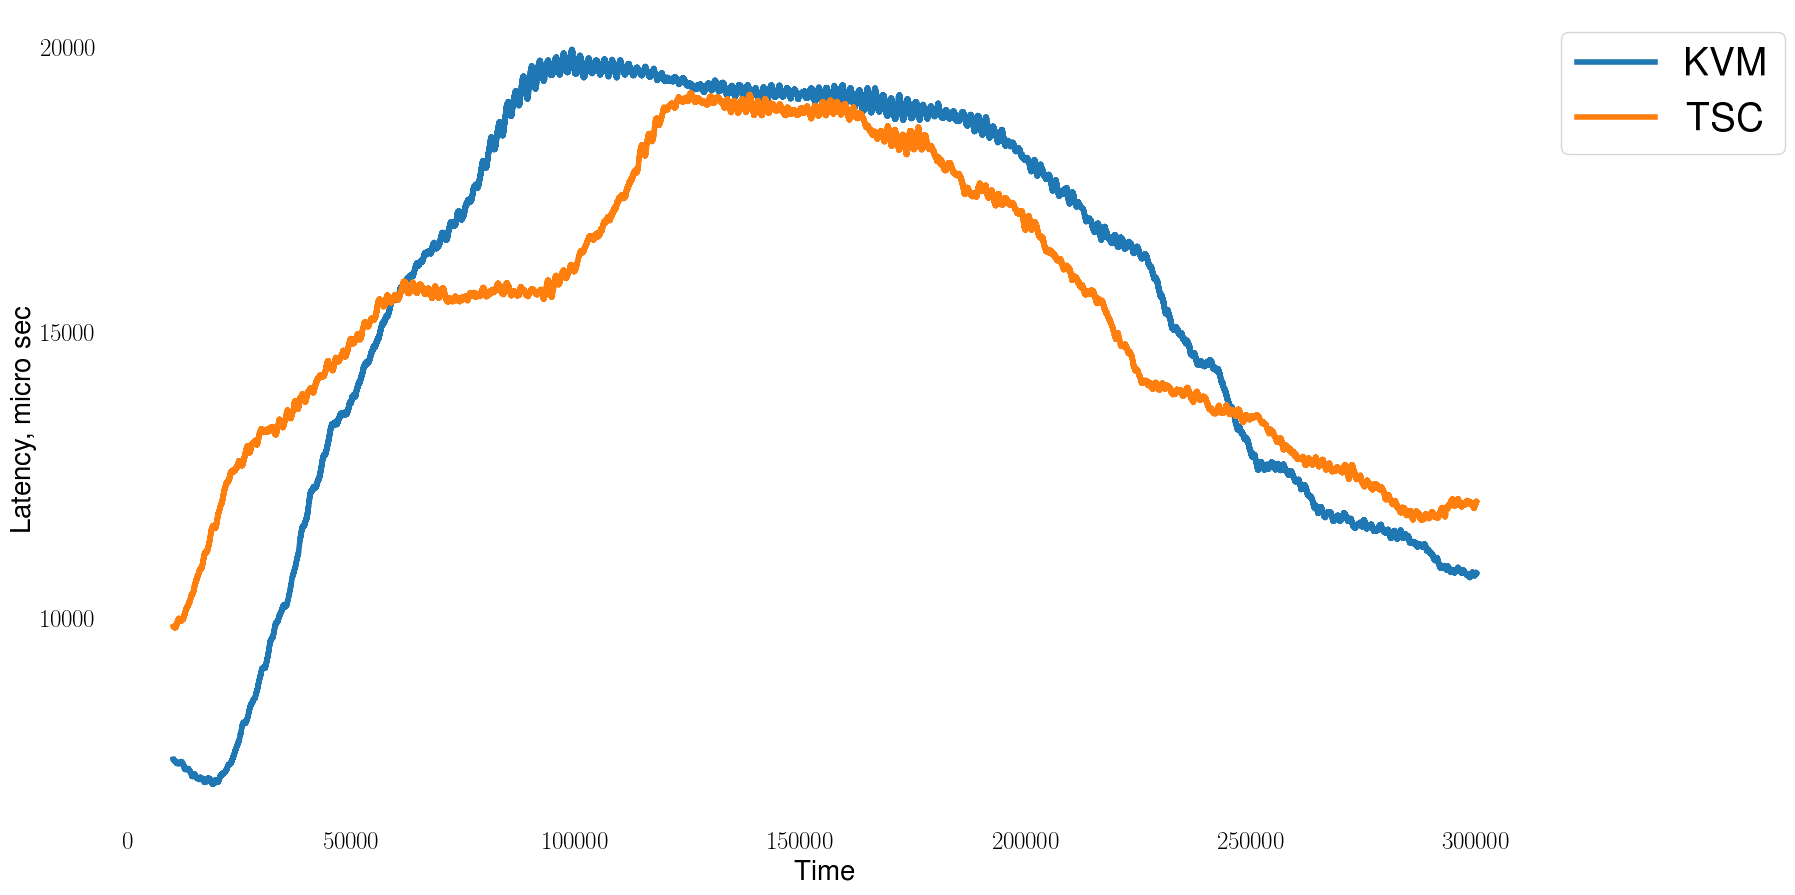
\includegraphics[width=0.9\textwidth,center]{checkpoint_dirty_pages.png}

    \end{center}
\end{frame}

\fontsize{13pt}{14}\selectfont
\section{Containers?}
\fontsize{17pt}{18}\selectfont

\begin{frame}
    \frametitle{}
    \begin{center}
    \textbf{cgroups controllers}

    \begin{columns}
    \begin{column}{0.5\textwidth}
        \begin{itemize}[label={\MVRightarrow}]
            \item cpu,cpuacct
            \item cpuset
            \item memory
            \item devices
            \item freezer
            \item net\_cls
            \item rdma
        \end{itemize}
    \end{column}
    \begin{column}{0.5\textwidth}
        \begin{itemize}[label={\MVRightarrow}]
            \item blkio
            \item perf\_event
            \item net\_prio
            \item hugetlb
            \item pids
            \item rdma
        \end{itemize}
    \end{column}
    \end{columns}

    \end{center}
\end{frame}

\begin{frame}
    \frametitle{}
    \begin{center}
    \textbf{CONFIG\_MEMCG\_KMEM}

        \begin{itemize}[label={\MVRightarrow}]
            \item Enabled in modern versions
            \item PostgreSQL requires contiguous memory \\ for shared buffers
            \item It's being allocated using slab
            \item memory.kmem.limit\_in\_bytes is too high
        \end{itemize}

    \end{center}
\end{frame}

\begin{frame}[fragile]{}
    \frametitle{}
    \begin{center}

        \begin{minted}[fontsize=\normalsize]{bash}
# Host, normal
 Zone: Normal
 Free KiB in zone: 807232.00
    Fragment size        Free fragments
    4096                 29612
    8192                 23308
    16384                13495

# Host with a container
 Zone: Normal
 Free KiB in zone: 109700.00
    Fragment size        Free fragments
    4096                 3405
    8192                 7082
    16384                1954
        \end{minted}

    \end{center}
\end{frame}

\begin{frame}
    \frametitle{}
    \begin{center}
    \textbf{Bad neighbor}

        \begin{itemize}[label={\MVRightarrow}]
            \item buddy allocator can fail \\ to find a page of proper size
            \item kernel will start a compaction process
            \item compaction implementation \\ knows nothing about cgroups
        \end{itemize}

    \end{center}
\end{frame}

\fontsize{13pt}{14}\selectfont
\section{Storage IO}
\fontsize{17pt}{18}\selectfont

\begin{frame}
    \frametitle{}
    \begin{center}
        \textbf{WAL}

        \vspace{1.0cm}

        \only<1>{
            \begin{tikzpicture}
                \draw[
                    -,
                    line width=0.75mm,
                    dashed
                ] (-1,-2.5) to (9,-2.5);

                \draw[
                    line width=0.5mm,
                    rounded corners=0.2cm,
                    pattern=north west lines,
                    pattern color=green!30
                    ] (-1,-3) rectangle (9,-4) node[pos=.5] {\textbf{storage}};

                \draw[
                    line width=0.5mm,
                    rounded corners=0.2cm,
                    fill=blue!30
                    ] (0,0) rectangle (2,1) node[pos=.5] {\textbf{client}};

                \draw[
                    line width=0.5mm,
                    rounded corners=0.2cm,
                    color=white
                    ] (3,0) rectangle (5,1) node[pos=.5] {};

                \draw[
                    line width=0.5mm,
                    rounded corners=0.2cm,
                    color=white
                    ] (6,0) rectangle (8,1) node[pos=.5] {};

                \draw[
                    line width=0.5mm,
                    rounded corners=0.2cm,
                    color=white
                    ] (0.5,-1) rectangle (1.5,-2) node[pos=.5] {};

            \end{tikzpicture}
        }

        \only<2>{
            \begin{tikzpicture}
                \draw[
                    -,
                    line width=0.75mm,
                    dashed
                ] (-1,-2.5) to (9,-2.5);

                \draw[
                    line width=0.5mm,
                    rounded corners=0.2cm,
                    pattern=north west lines,
                    pattern color=green!30
                    ] (-1,-3) rectangle (9,-4) node[pos=.5] {\textbf{storage}};

                \draw[
                    line width=0.5mm,
                    rounded corners=0.2cm,
                    fill=blue!30
                    ] (0,0) rectangle (2,1) node[pos=.5] {\textbf{client}};

                \draw[
                    line width=0.5mm,
                    rounded corners=0.2cm,
                    fill=gray!30
                    ] (0.5,-1) rectangle (1.5,-2) node[pos=.5] {\textbf{W}};

                \draw[
                    <-,
                    line width=0.75mm,
                ] (1,-1) to (1,0);

                \draw[
                    line width=0.5mm,
                    rounded corners=0.2cm,
                    color=white
                    ] (3,0) rectangle (5,1) node[pos=.5] {};

                \draw[
                    line width=0.5mm,
                    rounded corners=0.2cm,
                    color=white
                    ] (6,0) rectangle (8,1) node[pos=.5] {};

            \end{tikzpicture}
        }

        \only<3>{
            \begin{tikzpicture}
                \draw[
                    -,
                    line width=0.75mm,
                    dashed
                ] (-1,-2.5) to (9,-2.5);

                \draw[
                    line width=0.5mm,
                    rounded corners=0.2cm,
                    pattern=north west lines,
                    pattern color=green!30
                    ] (-1,-3) rectangle (9,-4) node[pos=.5] {\textbf{storage}};

                \draw[
                    line width=0.5mm,
                    rounded corners=0.2cm,
                    fill=blue!30
                    ] (0,0) rectangle (2,1) node[pos=.5] {\textbf{client}};

                \draw[
                    line width=0.5mm,
                    rounded corners=0.2cm,
                    fill=gray!30
                    ] (0.5,-1) rectangle (1.5,-2) node[pos=.5] {\textbf{W}};

                \draw[
                    <-,
                    line width=0.75mm,
                ] (1,-1) to (1,0);

                \draw[
                    line width=0.5mm,
                    rounded corners=0.2cm,
                    fill=blue!30
                    ] (3,0) rectangle (5,1) node[pos=.5] {\textbf{client}};

                \draw[
                    line width=0.5mm,
                    rounded corners=0.2cm,
                    color=white
                    ] (6,0) rectangle (8,1) node[pos=.5] {};

                \draw[
                    line width=0.5mm,
                    rounded corners=0.2cm,
                    fill=gray!30
                    ] (3.5,-1) rectangle (4.5,-2) node[pos=.5] {\textbf{W}};

                \draw[
                    <-,
                    line width=0.75mm,
                ] (4,-1) to (4,0);

            \end{tikzpicture}
        }

        \only<4>{
            \begin{tikzpicture}
                \draw[
                    -,
                    line width=0.75mm,
                    dashed
                ] (-1,-2.5) to (9,-2.5);

                \draw[
                    line width=0.5mm,
                    rounded corners=0.2cm,
                    pattern=north west lines,
                    pattern color=green!30
                    ] (-1,-3) rectangle (9,-4) node[pos=.5] {\textbf{storage}};

                \draw[
                    line width=0.5mm,
                    rounded corners=0.2cm,
                    fill=blue!30
                    ] (0,0) rectangle (2,1) node[pos=.5] {\textbf{client}};

                \draw[
                    line width=0.5mm,
                    rounded corners=0.2cm,
                    fill=gray!30
                    ] (0.5,-1) rectangle (1.5,-2) node[pos=.5] {\textbf{W}};

                \draw[
                    <-,
                    line width=0.75mm,
                ] (1,-1) to (1,0);

                \draw[
                    line width=0.5mm,
                    rounded corners=0.2cm,
                    fill=blue!30
                    ] (3,0) rectangle (5,1) node[pos=.5] {\textbf{client}};

                \draw[
                    line width=0.5mm,
                    rounded corners=0.2cm,
                    color=white
                    ] (6,0) rectangle (8,1) node[pos=.5] {};

                \draw[
                    line width=0.5mm,
                    rounded corners=0.2cm,
                    fill=gray!30
                    ] (3.5,-1) rectangle (4.5,-2) node[pos=.5] {\textbf{W}};

                \draw[
                    <-,
                    line width=0.75mm,
                ] (4,-1) to (4,0);

                \draw[
                    ->,
                    line width=0.75mm,
                ] (1.5,-1.5) to (3.5,-1.5);

                \draw[
                    ->,
                    line width=0.75mm,
                ] (4,-2) to (4,-3);

            \end{tikzpicture}
        }

        \only<5>{
            \begin{tikzpicture}
                \draw[
                    -,
                    line width=0.75mm,
                    dashed
                ] (-1,-2.5) to (9,-2.5);

                \draw[
                    line width=0.5mm,
                    rounded corners=0.2cm,
                    pattern=north west lines,
                    pattern color=green!30
                    ] (-1,-3) rectangle (9,-4) node[pos=.5] {\textbf{storage}};

                \draw[
                    line width=0.5mm,
                    rounded corners=0.2cm,
                    fill=blue!30
                    ] (0,0) rectangle (2,1) node[pos=.5] {\textbf{client}};

                \draw[
                    line width=0.5mm,
                    rounded corners=0.2cm,
                    fill=gray!30
                    ] (0.5,-1) rectangle (1.5,-2) node[pos=.5] {\textbf{W}};

                \draw[
                    <-,
                    line width=0.75mm,
                ] (1,-1) to (1,0);

                \draw[
                    line width=0.5mm,
                    rounded corners=0.2cm,
                    fill=blue!30
                    ] (3,0) rectangle (5,1) node[pos=.5] {\textbf{client}};

                \draw[
                    line width=0.5mm,
                    rounded corners=0.2cm,
                    fill=blue!30
                    ] (6,0) rectangle (8,1) node[pos=.5] {\textbf{writer}};

                \draw[
                    line width=0.5mm,
                    rounded corners=0.2cm,
                    fill=gray!30
                    ] (3.5,-1) rectangle (4.5,-2) node[pos=.5] {\textbf{W}};

                \draw[
                    <-,
                    line width=0.75mm,
                ] (4,-1) to (4,0);

                \draw[
                    ->,
                    line width=0.75mm,
                ] (1.5,-1.5) to (3.5,-1.5);

                \draw[
                    ->,
                    line width=0.75mm,
                ] (4.5,-1.5) to (7,-1.5);

                \draw[
                    ->,
                    line width=0.75mm,
                ] (7,0) to (7,-3);

            \end{tikzpicture}
        }

    \end{center}
\end{frame}

\begin{frame}
    \frametitle{}
    \begin{center}
    \textbf{WAL}

        \begin{itemize}[label={\MVRightarrow}]
            \item bgwriter write to WAl \\
                (transaction snaphots for replication)
            \item logical decoding write more data to WAL
        \end{itemize}

    \end{center}
\end{frame}

\begin{frame}
    \frametitle{}
    \begin{center}
    \textbf{NVMe}

        \begin{itemize}[label={\MVRightarrow}]
            \item better for resourse sharing (PCI express) \\
                under the virtualization
            \item /sys/block/sda/queue/scheduler [noop|none]
            \item DSM operations
        \end{itemize}

    \end{center}
\end{frame}

\begin{frame}
    \frametitle{}
    \begin{center}
    \textbf{NVMe DSM}

        \begin{itemize}[label={\MVRightarrow}]
            \item Expected lifetime
            \item Sequential write/read prepare
            \item Access frequency
        \end{itemize}

    \end{center}
\end{frame}

\begin{frame}
    \frametitle{}
    \begin{center}
    \textbf{DSM support}

        \begin{itemize}[label={\MVRightarrow}]
            \item Command DWORD 11 in ioctl
            \item fcntl SET\_FILE\_RW\_HINT
            \item nvme-cli
            \item Specify a start block and a range length
        \end{itemize}

        \normalsize{NVM Express Revision 1.3c May 24, 2018}

    \end{center}
\end{frame}

\begin{frame}[fragile]{}
    \frametitle{}
    \begin{center}

        \begin{minted}[fontsize=\normalsize]{bash}
# get a start block
hdparm --fibmap data_file
data_file:
 filesystem blocksize 4096, begins at LBA 0;
 assuming 512 byte sectors.
 byte_offset  begin_LBA    end_LBA    sectors
           0   55041560   55041567          8

# set dsm for sequential read optimized
nvme dsm /dev/nvme1n01 --idr --slbs=55041560 --blocks=8
        \end{minted}

    \end{center}
\end{frame}

\fontsize{13pt}{14}\selectfont
\section{Containers?}
\fontsize{17pt}{18}\selectfont

\begin{frame}
    \frametitle{}
    \begin{center}
    \textbf{bklio controller}

        \begin{itemize}[label={\MVRightarrow}]
            \item CFQ \& throttling policy (generic block layer)
            \item No weight related options will work without CFQ
            \item Advisable io scheduler for SSD is noop/none
            \item Block layer do sampling to enforce throttling
        \end{itemize}

    \end{center}
\end{frame}

\begin{frame}[fragile]{}
    \frametitle{}
    \begin{center}

        \vspace{0.3cm}
        \begin{minted}[fontsize=\normalsize]{bash}
8388   8388   postgres     blk_throtl_bio
        blk_throtl_bio+0x1        [kernel]
        dm_make_request+0x80      [kernel]
        generic_make_request+0xf6 [kernel]
        submit_bio+0x7d           [kernel]
        blkdev_issue_flush+0x68   [kernel]
        ext4_sync_file+0x310      [kernel]
        vfs_fsync_range+0x4b      [kernel]
        do_fsync+0x3d             [kernel]
        sys_fdatasync+0x13        [kernel]
        fdatasync+0x10            [libc-2.24.so]
        XLogBackgroundFlush+0x17e [postgres]
        WalWriterMain+0x1cb       [postgres]
        PostmasterMain+0xfea      [postgres]
        \end{minted}

    \end{center}
\end{frame}

\begin{frame}
    \frametitle{}
    \begin{center}
    \textbf{throttle\_sample\_time}

		\begin{flushleft}
		This is the time window that blk-throttle samples data, in millisecond.
		blk-throttle makes decision based on the samplings. Lower time means cgroups
		have more smooth throughput, but higher CPU overhead. This exists only when
		CONFIG\_BLK\_DEV\_THROTTLING\_LOW is enabled.
		\end{flushleft}

    \end{center}
\end{frame}

\begin{frame}
    \frametitle{}
    \begin{center}
    \textbf{blkio}

		\begin{flushleft}
		On traditional cgroup hierarchies, relationships between different controllers
		cannot be established making it impossible for writeback to operate accounting
		for cgroup resource restrictions and all writeback IOs are attributed to the
		root cgroup.

        \normalsize{\href{
            https://git.kernel.org/pub/scm/linux/kernel/git/torvalds/linux.git/commit/?h=v4.14-rc4&id=3e1534cf4a2a8278e811e7c84a79da1a02347b8b
        }{https://git.kernel.org/pub/scm/linux/kernel/git/torvalds/linux.git}}
		\end{flushleft}

    \end{center}
\end{frame}

\fontsize{18pt}{18}\selectfont
\begin{frame}
  \vspace*{2.5cm}
  \begin{minipage}[b][\paperheight]{\textwidth}
  \begin{center}

      %\raggedright%
      \linespread{1.0}%
      \usebeamerfont{title}%
      \usebeamercolor[fg]{title}%
      \if@noSmallCapitals%
        Questions?
      \else%
        \scshape{\color{black} Questions?}%
      \fi%
      \vspace*{0.3em}

      \usebeamerfont{subtitle}%
      \fontsize{13pt}{14}\selectfont
      \usebeamercolor[fg]{subtitle}%
        \begin{itemize}[label={}]
            \item {\color{black} \github\ github.com/erthalion}
            \item {\color{black} \twitter\ @erthalion}
            \item {\color{black}\email\ dmitrii.dolgov at zalando dot de}
            \item {\color{black}\email\ 9erthalion6 at gmail dot com}
        \end{itemize}
      \vspace*{2.5em}%

    \vfill
    \vspace*{2em}
  \end{center}
  \end{minipage}

\end{frame}

\end{document}
